\documentclass{beamer}
%Для защит онлайн лучше использовать разрешение 16x9
%\documentclass[aspectratio=169]{beamer}

\usepackage{beamerthemesplit}
\usepackage{wrapfig}
\usetheme{SPbGU}
\usepackage{pdfpages}
\usepackage{amsmath}
\usepackage{cmap} 
\usepackage[T2A]{fontenc} 
\usepackage[utf8]{inputenc}
\usepackage[english,russian]{babel}
\usepackage{indentfirst}
\usepackage{amsmath}
\usepackage{tikz}
\usepackage{multirow}
\usepackage[noend]{algpseudocode}
\usepackage{algorithm}
\usepackage{algorithmicx}
\usetikzlibrary{shapes,arrows}
\usepackage{fancyvrb}
\usepackage{appendixnumberbeamer}

\newtheorem{rutheorem}{Теорема}
\newtheorem{ruproof}{Доказательство}
\newtheorem{rudefinition}{Определение}
\newtheorem{rulemma}{Лемма}

\beamertemplatenavigationsymbolsempty

% То, что в квадратных скобках, отображается внизу по центру каждого слайда. 
\title[Параллелизация miniKanren]{Параллельная реализация miniKanren}

% То, что в квадратных скобках, отображается в левом нижнем углу. 
\institute[СПбГУ]{}

% То, что в квадратных скобках, отображается в левом нижнем углу.
\author[Андрей Диденко]{Андрей Антонович Диденко, Б-07.21 ММ }
 
\begin{document}
{
\setbeamertemplate{footline}{}
% Лого университета или организации, отображается в шапке титульного листа
\begin{frame}
  
\includegraphics[width=1.4cm]{pictures/SPbGU_Logo.png}
  \vspace{-35pt}
  \hspace{-10pt}
  \begin{center}
    \begin{tabular}{c}
      \scriptsize{Санкт-Петербургский государственный университет} \\
      \scriptsize{Кафедра системного программирования}
    \end{tabular}
    \titlepage
  \end{center}

  \btVFill

  {\scriptsize
    % У научного руководителя должна быть указана научная степень
    {\bfseries Научный руководитель:} Д.С.Косарев, ассистент кафедры системного программирования \\
    % Консультанта может и не быть. Должна быть указана должность или ученая степень
    % {\bfseries Консультант:}  к.ф.-м.н. Д.С.Косарев, "MatMex, JetBrains Research laboratory" \\
    % Для курсовой не обязателен. Должна быть указана должность или ученая степень
    % {\bfseries Рецензент:} д.т.н., проф. И.И. Иванов, исполнительный директор ООО ``Рога и копыта''
  }
  \begin{center}
    \vspace{5pt}
    \scriptsize{Санкт-Петербург\\
      2022}
  \end{center}

\end{frame}
}

\begin{frame}[fragile]
  \frametitle{Введение}
  \begin{itemize}
    \item Работа направлена на повышение эффективности вычислений на языке miniKanren путем декомпозиции задачи на потоках
          % Краткий обзор тематики работы (как вариант --- устно, пока показывается титульный слайд)
    \item Данное решение предназначено для разработчиков, иcпользующих miniKanren
          % Не нужно определять общеизвестные понятия
    \item Сообщество miniKanren всерьез еще этим не занималось, поэтому у работы нет аналогов
          % Применимость/полезность данной работы, обоснование выбора именно этой темы
          % \item Если тема похожа на темы других работ (в том числе прошлых лет), надо явно описать разницу
  \end{itemize}
\end{frame}


\begin{frame}
  \frametitle{Постановка задачи}
  \textbf{Целью} работы является распараллеливание miniKanren %озвученной выше  

  \textbf{Задачи}:
  \begin{itemize}
    % \item Выбрать алгоритм, подход, метод %основываясь на проведённом анализе проблемы, области, существующих решений
          % \item Доказать корректность алгоритма
    \item Выбрать версию OCaml, на которой будет реализована параллельность 
    %\item Изучить примеры параллелизации
    \item Научиться параллелить две независимые задачи на miniKanren
    \item Подзадачи:
    \begin{itemize}
      % \item Выбрать алгоритм, подход, метод %основываясь на проведённом анализе проблемы, области, существующих решений
            % \item Доказать корректность алгоритма
      \item запустить параллельно appendo
      %\item Изучить примеры параллелизации
      \item запустить параллельно reverso
      \item Объединить поток Stream в ответ
    \end{itemize}
  \end{itemize}
\end{frame}




\begin{frame}
  \frametitle{Используемые инструменты, подходы}
  \begin{itemize}
    \item За основу взят язык программирования OCaml, а также встаиваемый в него язык miniKanren
    \item Для разработки моего проекта была задействована библиотека Domainslib для OСaml версии 5
    \item В 5 версии добавлены новые инструменты для параллелизации 
  \end{itemize}

\end{frame}

% \begin{frame}
%   \frametitle{Существующие решения}
%   Возможно, предметная область сложна и потребуется больше одного слайда, но затягивать введение не стоит. Постарайтесь уложиться в 1--2 слайда
%   \begin{itemize}
%     \item Выводы
%           \begin{itemize}
%             \item Подвести итог
%             \item Указать недостатки существующих подходов, на борьбу с которыми
%                   направленна данная работа
%             \item Чётко сформулировать существующую проблему, которая будет решаться в данной работе
%           \end{itemize}
%   \end{itemize}
% \end{frame}


% Обязательный слайд: четкая формулировка цели данной работы и постановка задачи
% Описание выносимых на защиту результатов, процесса или особенностей их достижения и т.д.
%Идеально, если есть по одному слайду на каждую поставленную задачу            

\begin{frame}
  \frametitle{OCaml}
  \begin{itemize}
  \item Выбрана самая свежая версия OCaml (5.0.0~beta2)\footnote{\url{https://ocaml.org/news/ocaml-5.0.beta2}(Дата доступа: 08.12.22)}
  В этой версии добавили multicore в runtime и
  c помощью этого легко параллелить программы на OCaml
  \item Почему была выбрана 5 версия? В 4 версии нет настоящего параллелизма (приходится запускать системные потоки и параллельность происходит на уровне системы, а не на уровне OCaml)
  \end{itemize}
\end{frame}


% \begin{frame}
%   \frametitle{Алгоритм распараллеливания}
%   \begin{itemize}
%     \item 1.Рассматривая реализацию миниканрен на окамл,которая называется unicanren,
%           придём к выводу, что можно распараллелить функцию Conde.
%     \item При попытке параллелить функцию eval, результаты оказались отрицательным
%     \item Делаем вывод,что необходимо параллелить run. Хотим доставать ответы по мере поступаления изнутри функции и вытягивать их на верхний уровень(в ответ)
%   \end{itemize}
% \end{frame}

  
\begin{frame}
  \frametitle{DomainsLib}
  % Задается ширина столбцов
  \begin{itemize}
  \item Для распараллеливания используется библиотека DomainsLib\footnote{\url{https://github.com/ocaml-multicore/parallel-programming-in-multicore-ocaml}(Дата доступа: 08.12.22)}, 
  в которой присутствуют 2 модуля: Task -- для вызова многопоточности и Chan -- для передачи информации между доменами
  \item Для освоения способов применения я изучил предложенные примеры параллельного сложения матриц и также рассмотрел реализацию чисел Фибоначчи, которая тоже была распараллелена
  \end{itemize}
\end{frame}


% \begin{frame}[fragile]
%   \frametitle{Доказательство корректности алгоритма}
%   {\tiny Формулировки утверждений. Идеи доказательств проговариваются устно.}
%   \begin{rutheorem}[Пифагора: геометрическая формулировка]
%     В прямоугольном треугольнике площадь квадрата, построенного на гипотенузе, равна сумме площадей квадратов, построенных на катетах.
%   \end{rutheorem}

%   \begin{rutheorem}[Пифагора: алгебраическая формулировка]
%     В прямоугольном треугольнике квадрат длины гипотенузы равен сумме квадратов длин катетов.

%     То есть, если обозначить длину гипотенузы треугольника через $c$, а длины катетов
%     через $a$ и $b$, получим верное равенство: $a^2 + b^2 = c^2$.
%   \end{rutheorem}

%   \begin{rutheorem}[Обратная теорема Пифагора]
%     Для всякой тройки положительных чисел a, b и c, такой, что $a^2 + b^2 = c^2$, существует прямоугольный треугольник с катетами a и b и гипотенузой c.
%   \end{rutheorem}
% \end{frame}

\begin{frame}
  \frametitle{Unicanren}
  \begin{itemize}
  \item Вся проделанная работа выполнена на минимальной реализации miniKanren -- Unicanren\footnote{{https://github.com/Kakadu/unicanren}(Дата доступа: 08.12.22)}, которая состоит из 4 базовых конструкций: Fresh, Unify, Conde и Conj
  \item В этой работе есть возможность параллелить только дизъюнкцию (conde), так как это выполнение двух независимых задач, в то время как все остальное - зависимые задачи и нет осознания того, как их параллелить
  
  \end{itemize}
  \end{frame}

% \begin{frame}[fragile]
%   \frametitle{Архитектура решения}
%   \begin{itemize}
%     \item В реализации интересны архитектура, библиотеки, инструменты
%     \item Не надо добавлять на слайд примеры кода
%   \end{itemize}
%   \begin{center}
%     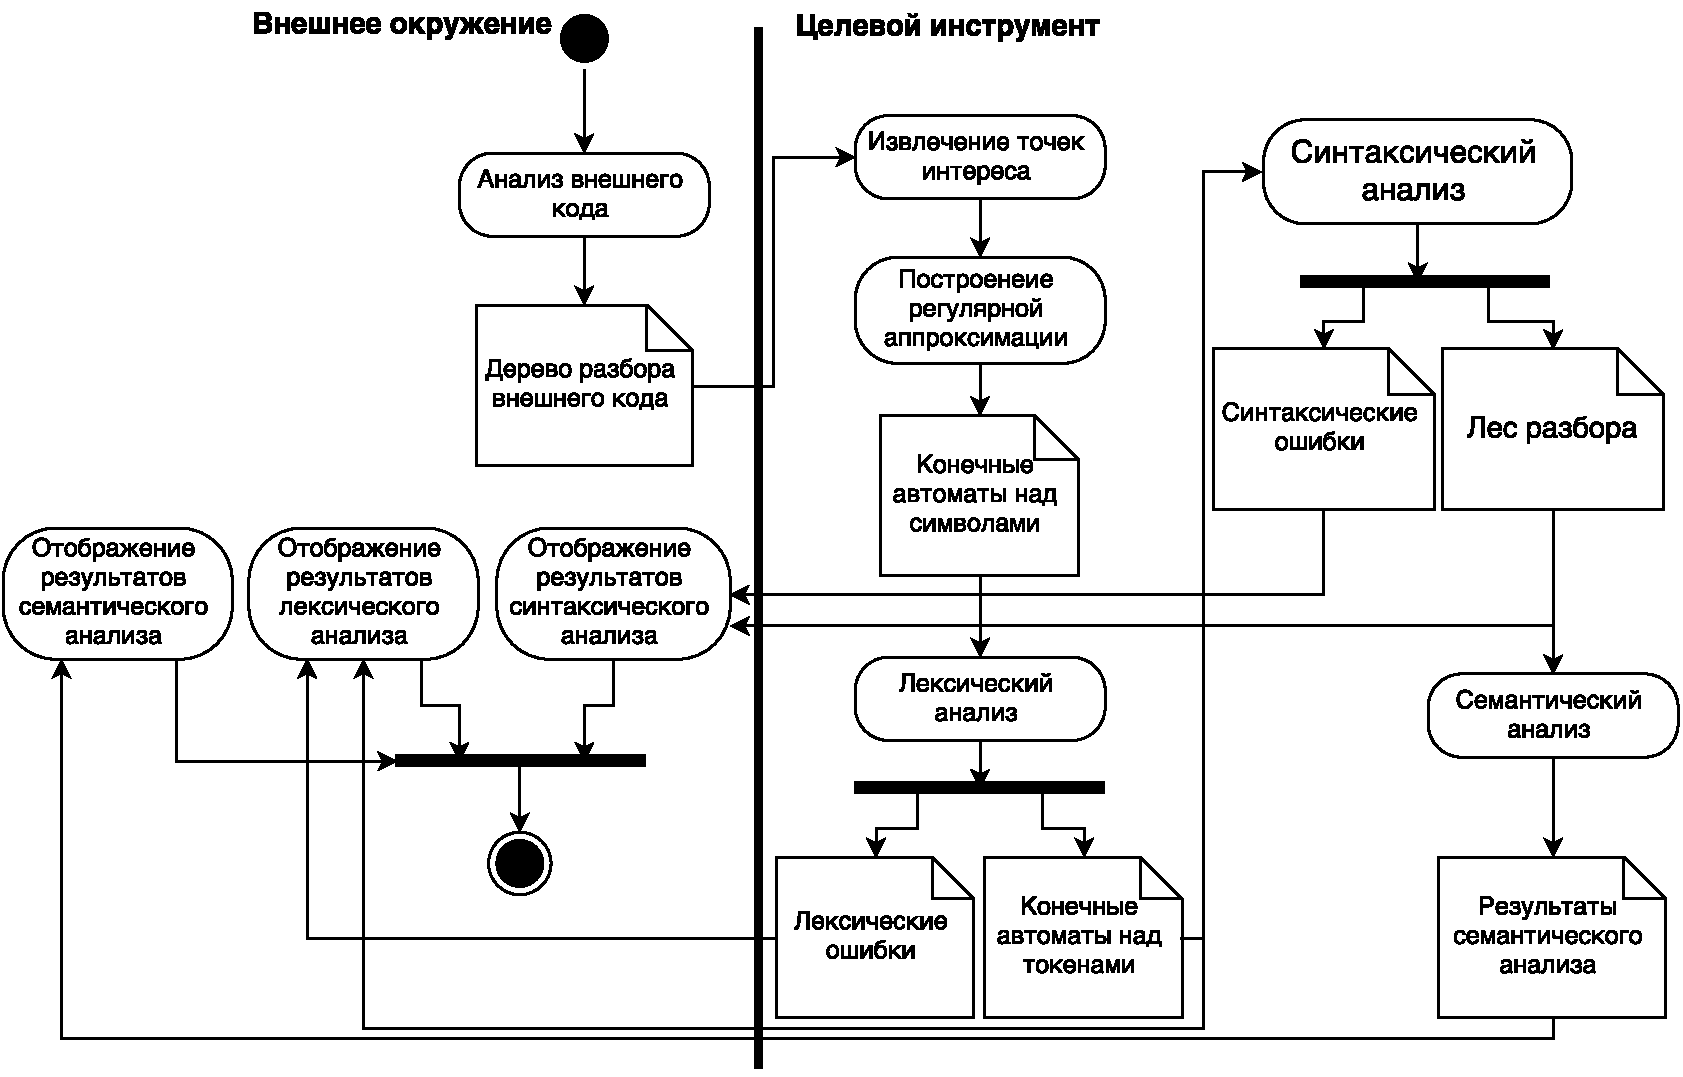
\includegraphics[width=0.8\textwidth]{pictures/Activ_SEL_Processing.pdf}
%   \end{center}
% \end{frame}

\begin{frame}
  \frametitle{Процесс работы}
  \begin{itemize}
  \item Так как для меня не только miniKanren, но и язык OCaml оказались неизведанными, мне пришлось помучиться для их освоения
  \item Я начал с простых задач:
  \begin{itemize}
  \item Параллельный запуск appendo
  \item Параллельный запуск reverso (при котором возникла проблема нехватки памяти)
  \item Параллельный запуск некоторых функций, которые возвращают несколько ответов
  \item Последней задачей оказалось слияние Stream'ов: Хотим доставать ответы по мере поступаления изнутри функции и вытягивать их на верхний уровень(в ответ)
  \end{itemize}
  \end{itemize}
  \end{frame}

% \begin{frame}[t]
%   \frametitle{Экспериментальное исследование}
%   Постановка эксперимента
%   \begin{itemize}
%     \item На каком наборе данных проводилось экспериментальное исследование, почему были выбраны именно эти данные
%     \item На каком оборудовании проводилось исследование
%     \item Какие решения были выбраны для сравнения и почему
%   \end{itemize}
% \end{frame}

\begin{frame}[t]
  \frametitle{Дальнейшие планы}
  \begin{center}
    \item Сделать параллельно исполняющуюся реализацию miniKanren
  \end{center}
  
  \end{frame}

% \begin{frame}[t]
%   \frametitle{Результаты экспериментального исследования}
%   \begin{itemize}
%     \item Какие результаты показало экспериментальное исследование
%     \item Желательно привести графики, иллюстрирующие полученные результаты
%           \begin{itemize}
%             \item У иллюстраций должны быть подписи, у графиков --- легенда, подписи к осям, например:
%           \end{itemize}
%   \end{itemize}
%   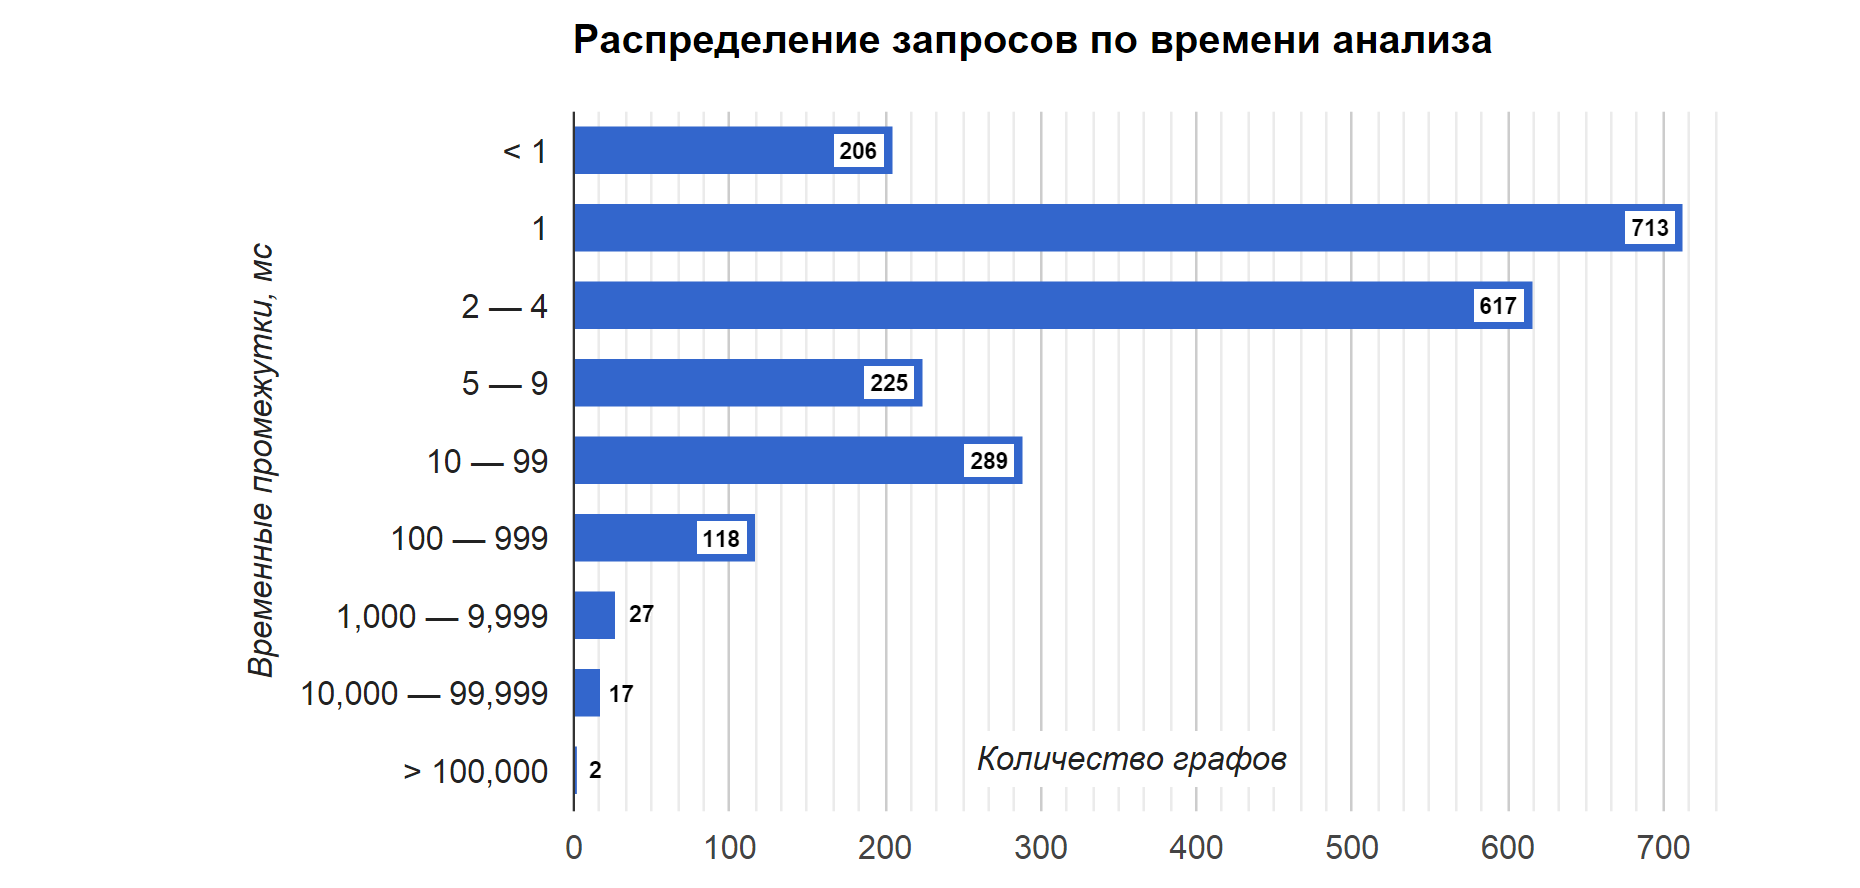
\includegraphics[width=10cm]{pictures/dist.png}
% \end{frame}


% \begin{frame}
%   \frametitle{Результаты}
%   \begin{itemize}
%     \item Практически то же, что и на слайде с постановкой задачи, но в совершенной форме --- что делал лично автор
%     \item Четкое отделение результатов своей работы (особенно для коллективных работ)
%     \item Формулировать глаголами совершенного вида в прошедшем времени (``сделано'', ``получено'')
%     \item Обсуждение (ограничения, валидность, альтернативы)
%     \item Не нужно слайдов типа ``Все'', ``Вопросы?'', ``Спасибо за внимание''
%   \end{itemize}

%   \begin{itemize}
%     \item Если результаты были представлены на конференции и опубликованы, это желательно указать
%   \end{itemize}
% \end{frame}

\begin{frame}
  \frametitle{Результаты}
  \begin{itemize}
  \item Выбрал 5 версию OCaml для реализации
  %\item Изучил примеры параллелизации
  \item Научился параллельно запускать 2 независимые задачи
  \item Подготовился к реализации настоящего интерпретатора\footnote{\url{https://github.com/K0lba/unicanren} (Дата доступа: 07.12.22)}
  \end{itemize}
  
  
  \end{frame}
  


%\addtocounter{framenumber}{1}
\appendix


\end{document}